\documentclass{classrep}
\usepackage[utf8]{inputenc}
\frenchspacing

\usepackage{graphicx}
\usepackage[usenames,dvipsnames]{color}
\usepackage[hidelinks]{hyperref}
\usepackage{lmodern}
\usepackage{placeins}
\usepackage{url}
\usepackage{amsmath, amssymb, mathtools}
\usepackage{listings}
\usepackage{fancyhdr, lastpage}

\pagestyle{fancyplain}
\fancyhf{}
\renewcommand{\headrulewidth}{0pt}
\cfoot{\thepage\ / \pageref*{LastPage}}

%--------------------------------------------------------------------------------------%
\studycycle{Applied Information Technology, 2 cycle}
\coursesemester{II}

\coursename{Soft Computing Laboratory}
\courseyear{2021/2022}

\courseteacher{dr inż. Kamil Stokfiszewski}
\coursegroup{Wednesday, 8:30}

\author{%
    \studentinfo[239671@edu.p.lodz.pl]{Jan Karwowski}{239671}\\
    \studentinfo[239676@edu.p.lodz.pl]{Kamil Kowalewski}{239676}\\
}

\title{Assignment 1.: The Delta rule}

\begin{document}
    \maketitle
    \thispagestyle{fancyplain}

    \tableofcontents
    \newpage

    \section{Main goal}
    \label{main_goal} {
        The main goal of this task is to prepare implementation of single linear neuron.
        For training the delta rule has to be used in two variants, the first one is
        with single training patterns and the second one is with multiple training
        patterns.
    }

    \section{Theoretical background}
    \label{theory} {
        \begin{figure}[!htbp]
            \centering
            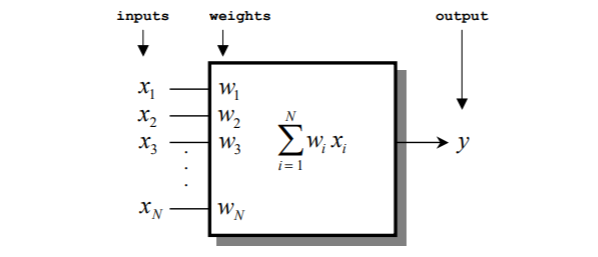
\includegraphics[width=\textwidth]{img/linear_neuron.png}
            \caption{Simple, linear artificial neuron}
            \label{artificial_neuron}
        \end{figure}
        \FloatBarrier

        The concept of artificial neuron (fig. \ref{artificial_neuron}) and its
        learning method, called ,,delta rule'' was invented many years ago. It is very
        simple and based on dot product of input values and trainable parameters called
        ,,weights''. These weights are modified during training process, to make output
        of neuron closer to the desired value (for particular input). The following
        equation presents delta rule:
        \begin{equation}
            w_{i} = w_{i} + \ni (z - y) x_{i}
        \end{equation}
        where $i$ is the number of input and its corresponding weight, $x_i$ is an
        input, $w_i$ is a weights, $y$ stands for neuron output and $z$ for desired
        output. $\ni$ is a so called ,,learnig rate'', which determines learning speed.
    }

    \section{Implementation details}
    \label{implementation} {
        Program was written in Python programming language and very popular numpy
        library was used as well. Training patterns and weights were stored as vectors
        (one-dimensional arrays) and only required operations were addition and
        multiplication. Since the whole source code consists of no more then few lines
        it definitely does not require more explanation.
    }

    \section{Experiments and results}
    \label{results} {
        This section presents simulation results for single pattern case and multiple
        pattern case. There are six mutable parameters, which was changed between
        experiments:

        \begin{itemize}
            \item the number of neuron's inputs - N
            \item the number of training epochs - K
            \item training step - $\eta$
            \item the interval, which the initial weights should be randomly chosen from -
            $[\omega_{1}, \omega_{2}]$
            \item the interval, which the training pattern's inputs should be randomly
            \item chosen
            from - $[\rho_{1}, \rho_{2}]$
            \item the number of training patterns - P (only for multiple pattern case)
        \end{itemize}

        \subsection{Single pattern experiments}
        \label{results:single} {
            Table \ref{tab:results:single} presents results for series of experiments
            related to single pattern training. Each row corresponds to single
            experiment. Single experiment is a single training attempt, where all the
            parameters are immutable and given number of epochs (training loops) are
            processed.

            \begin{table}[!htbp]
                \centering
                \begin{tabular}{|c|c|c|c|c|c|c|c|}
                    \hline
                    & N & K & $\eta$ & $[\omega_{1}, \omega_{2}]$ & $[\rho_{1},
                    \rho_{2}]$ & $y$ & $z$ \\ \hline
                    1 & 10 & 100 & 0.1 & $[-1,1]$ & $[-1,1]$ & -0.448 & -0.448 \\ \hline
                    2 & 10 & 100 & 0.01 & $[-1,1]$ & $[-1,1]$ & -0.448 & -0.5237 \\ \hline
                    3 & 10 & 100 & 0.001 & $[-1,1]$ & $[-1,1]$ & -0.448 & -0.9791 \\
                    \hline
                    4 & 10 & 10000 & 0.001 & $[-1,1]$ & $[-1,1]$ & -0.448 & -0.488 \\
                    \hline
                    5 & 10 & 100 & 0.9 & $[-1,1]$ & $[-1,1]$ & -0.448 & -5.0504e+19 \\
                    \hline
                    6 & 100 & 100 & 0.1 & $[-1,1]$ & $[-1,1]$ & 0.101 & -7.9471e+29 \\
                    \hline
                    7 & 100 & 100 & 0.01 & $[-1,1]$ & $[-1,1]$ & 0.101 & 0.101 \\ \hline
                    8 & 100 & 100 & 0.01 & $[-100,100]$ & $[-1,1]$ & 0.101 & 0.101 \\
                    \hline
                    9 & 100 & 100 & 0.0001 & $[-100,100]$ & $[-100,100]$ & 10.0999 & 3
                    .0001e+149 \\ \hline
                \end{tabular}
                \caption{Experiment results for single pattern training}
                \label{tab:results:single}
            \end{table}
            \FloatBarrier
        }

        \subsection{Multiple pattern experiments}
        \label{results:multiple} {
            During the second series of experiments, related to multiple pattern
            training, we fixed all parameters except $P$ (number of training patterns)
            to values presented in table\ref{tab:results:multiple:params}. Number of
            training patterns changes between experiments as an explored variable. It
            should be considered in compare to $N$ value(number of inputs), which is
            fixed to 5.

            \begin{table}[!htbp]
                \centering
                \begin{tabular}{|c|c|c|c|c|}
                    \hline
                    N & K & $\eta$ & $[\omega_{1}, \omega_{2}]$ & $[\rho_{1},\rho_{2}]$ \\ \hline
                    5 & 10000 & $0.1$  & $[-1,1]$ & $[-1,1]$ \\ \hline
                \end{tabular}
                \caption{Fixed parameters' values for multiple training pattern
                experiments}
                \label{tab:results:multiple:params}
            \end{table}
            \FloatBarrier

            Results of experiments are presented in tables \ref{tab:results:multiple:m3},
            \ref{tab:results:multiple:m5} and \ref{tab:results:multiple:m6}.

            \begin{table}[!htbp]
                \centering
                \begin{tabular}{|c|c|}
                    \hline
                    z & y \\ \hline
                    -0.3556 & -0.3556 \\
                    -0.629 & -0.629 \\
                    0.8344 & 0.8344 \\ \hline
                \end{tabular}
                \caption{Experiment results for 3 patterns training}
                \label{tab:results:multiple:m3}
            \end{table}
            \FloatBarrier

            \begin{table}[!htbp]
                \centering
                \begin{tabular}{|c|c|}
                    \hline
                    z & y \\ \hline
                    0.3919 & y = 0.3919 \\
                    0.1061 & y = 0.1061 \\
                    0.8705 & y = 0.8705 \\
                    0.0252 & y = 0.0252 \\
                    -0.6448 & y = -0.6448 \\ \hline
                \end{tabular}
                \caption{Experiment results for 5 patterns training}
                \label{tab:results:multiple:m5}
            \end{table}
            \FloatBarrier

            \begin{table}[!htbp]
                \centering
                \begin{tabular}{|c|c|}
                    \hline
                    z & y \\ \hline
                    0.0737 & 0.0726 \\
                    -0.4131 & -0.3817 \\
                    -0.9788 & -1.0094 \\
                    0.7676 & 0.8055 \\
                    0.3128 & 0.3175 \\
                    0.8845 & 0.8322 \\ \hline
                \end{tabular}
                \caption{Experiment results for 6 patterns training}
                \label{tab:results:multiple:m6}
            \end{table}
            \FloatBarrier
        }
    }

    \section{Summary and conclusions}
    \label{summary} {
        Meaning and importance of each training parameter can be found basing on table
        \ref{tab:results:single}. The first four rows presents the impact of learning
        rate. The smaller it is the more time (epochs) is required to train neuron
        effectively. As shown in the fifth row, it must not be too much because
        algorithm may not converge. On the other hand, sometimes it is required to use
        lower learning rate (rows six and seven), because of too complicated
        optimization problem (many many inputs). This is a kind of a trade-off between
        speed and accuracy - lower learning rate requires more epochs to converge but is
        more accurate, higher learning rate converge faster but may be applied only to
        simpler problems. Last two rows are related to initialization intervals. We can
        see that initial weights values may be larger and algorithms still converge. In
        fact, weights are modified in time and become much more closer to the desired
        value in first few steps. The situation changes when we explore inputs initial
        interval. These values, which stays constant during training, are very
        sensitive and should be normalized before training. If they are too much,
        algorithm is not able to converge (learning steps are not precise enough). We
        can try to fix it using very low learning rate, but it may not help.

        In the second series of experiments we focus on relation between number of
        training patterns(M) and number of neuron's inputs (N). Number of inputs was
        fixed to value of 5. Number of training patterns takes three values: 3, 5, and
        6. Observations from experiments, presented in tables
        \ref{tab:results:multiple:m3}, \ref{tab:results:multiple:m5} and
        \ref{tab:results:multiple:m6} are pretty straightforward. Neuron is able to
        learn number of patterns, which is lower or equal to number of input. Where
        there is more "independent" training patterns then inputs, it is not possible
        to find perfect weights' values. It can be easily explained when considered
        artificial neuron training as solving system of $P$ (number of training
        patterns) linear equations with $N$ (number of inputs) variables, where each
        training pattern is a single linear equation. If training patterns are linearly
        independent(which is almost 100\% sure for random patterns), then there is:

        \begin{itemize}
            \item infinite set of solutions for $N > P$
            \item exactly one solution for $N = P$
            \item no solution for $N < P$
        \end{itemize}
    }


    \begin{thebibliography}{0}
        % @formatter:off
        \bibitem{instruction}{Labolatory instruction, URL: https://ftims.edu.p.lodz.pl/pluginfile.php/75436/\\mod\_resource/content/3/soft\_comp\_lab\_01\_DELTA.pdf}
        % @formatter:on
    \end{thebibliography}

\end{document}
